\begin{problem}[10]
若溢洪道的断面为三角形, 讨论溢洪流量.
\end{problem}
% --------------------------------------------------------------------
\begin{solution}
\begin{minipage}[c]{0.8\linewidth}
溢洪流量与流体的密度$\rho$, 重力加速度$g$, 上游水头$h$及三角形的顶角$\alpha$有关, 溢过三角形断面的流量为$Q$, 则有
\[
Q = f(\rho, g, h, \alpha)
\]
\end{minipage}
\begin{minipage}[c]{0.2\linewidth}
\begin{center}
\usetikzlibrary{calc,intersections,through,backgrounds}
\usetikzlibrary{decorations.pathreplacing,decorations.pathmorphing,arrows}
\begin{tikzpicture}
\coordinate (p1) at (0.6,0.2);
\coordinate (p2) at  (1.2,0.4);
\coordinate (p4) at (2,-0.2);
\coordinate (p6temp) at (2.5,1);
\coordinate (p7) at (3,1);
\path [name path=D] (p1)--(3,1);
\path [name path=E] (p4)--(p6temp);
\path [name intersections={of=D and E, by=p6}];

\coordinate (pd1) at (0,-0.4);
\path [name path=A] (pd1)--(3.9,0.9);
\path [name path=B] (p2)--(p4);
\path [name intersections={of=A and B, by=p3}];
\path [name intersections={of=A and E, by=p5}];

\draw[thick] (p1) -- (p2)--(p3)--(p4)  (p5)-- (p6)--(p7);
\draw[dashed, thick] (p4)--(p5);

\draw[dashed, thick] (p1)++(0,-0.4)--(p3) (p7)++(0,-0.4) -- (p5);

\draw[thick](p1)++(0,-0.9)--(p4);

\node at (1.55,0.125) {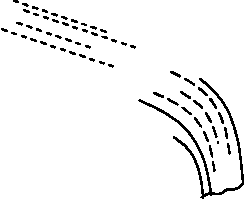
\includegraphics[width=60pt]{water.pdf}};
\draw[ <->,>=stealth',thick,blue](1,-0.09) -- (1,-0.55) node[right=-1pt, midway]{$h$};
\draw[ <->,>=stealth',thick,blue](p5) arc(80:138:0.707);
\node[blue] at (1.8,0.5) {$\alpha$};
\node[blue] at (1.25,1) {$\rho$};
\node[blue] at (2.0,-0.75) {$Q$};
\draw [blue,->,>=stealth',thick] (3,0.25) -- (3, -0.5) node [below]{$g$};
\end{tikzpicture}

\end{center}
\end{minipage}
上式中的各物理量的量纲分别为: $[Q]=MT^{-1}$, $[\rho]=ML^{-3}$, $[g]=LT^{-2}$, $[h]=L$, 而$\alpha$为无量纲量. 选取$\rho$, $g$, $h$三个量作为基本量, 且作为本问题的单位系统, 用以度量问题中的各量. 于是, 得到各量的量值所满足的关系
\[
\frac{Q}{\rho h^3 \sqrt{g/h}} = f(1,1,1,\alpha) \qquad \Longrightarrow \qquad Q = \rho g^{1/2} h^{5/2}f(\alpha)
\]
\end{solution}
